\section{Theory}

Sequential Logic circuits can be used to build more complex circuits like counters, shift registers, latches or memories, but for these types of circuits to operate in a sequential manner, they require some kind of a clock pulse or timing signal which can cause them to change their state. Clock pulses are generally square-shaped waves that
are produced by a single pulse generator circuit such as a Multivibrator which oscillates
between a \verb|HIGH| and a \verb|LOW| state. Sequential logic circuits that use the
clock signal for synchronization change their state on either the rising or falling
edge, or both of the clock signal.

A duty cycle or power cycle is the fraction of one period in which a signal or system is active. Generally, these signals have an even 50\% duty cycle, i.e.
it has a 50\% \verb|ON| time and a 50\% \verb|OFF| time.  There are basically three types of pulse
generation circuits depending on the number of stable states,

\begin{itemize}
    \item \textbf{Astable} has no stable states — it continually switches from one state to the other at a fixed frequency.
    \item \textbf{Monostable} in which one of the states is stable, but the other state is unstable (or transient). A trigger pulse causes the circuit to enter the unstable state. After entering the unstable state, the circuit will return to the stable state after a set time. Such a circuit is useful for creating a timing period of fixed duration in response to some external event.
    \item \textbf{Bistable} in which the circuit is stable in either state. It can be flipped from one state to the other by an external trigger pulse.
\end{itemize}

\subsection*{IC 555 Timer}
Initially called the "The IC Time Machine", the 555 timer is an integrated circuit used in a variety of timer, delay, pulse generation, and oscillator applications and is one of the most popular timing ICs.

\begin{figure}[H]
    \centering
    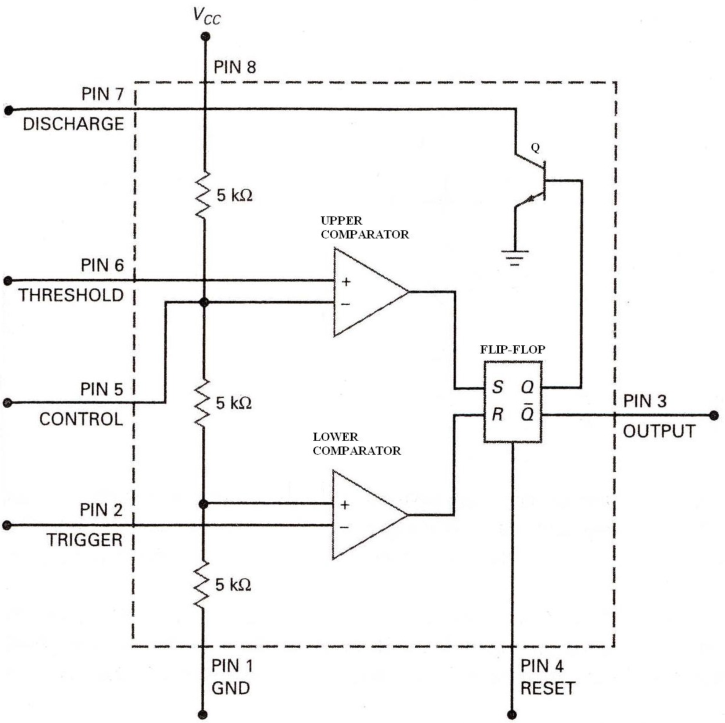
\includegraphics[width=0.90\columnwidth]{images/555a.png}
    \caption{Functional block diagram of IC 555}
    \label{fig:0}
\end{figure}

The 555 time typically comes with 8 pins:
\begin{itemize}[itemsep=10pt]
    \item [Pin 1:] \textit{(Ground)} All voltages are measured with respect to this terminal.
    \item [Pin 2:] \textit{(Trigger)} The output of the timer depends on the amplitude of the external trigger pulse applied to this pin. When a negative going pulse of amplitude greater than $1/3\,V_{CC}$ is applied to this pin, the output of the timer high. The output remains high as long as the trigger terminal is held at a low voltage.
    \item [Pin 3:] \textit{(Output)} The output of the timer is measured with respect to ground. There are
    two ways by which a load can be connected to the output terminal -- either between pin 3
    and ground or between pin 3 and supply voltage $+V_{CC}$. When the output is low the load
    current flows through the load connected between pin 3 and $+V_{CC}$ into the output terminal
    and is called \textit{sink current}. The current through the grounded load is zero when the output
    is low. For this reason the load connected between pin 3 and $+V_{CC}$ is called the \textit{normally
    on load} and that connected between pin 3 and ground is
    called \textit{normally off-load}. On the other hand, when the output is high the current through
    the load connected between pin 3 and $+V_{CC}$ is zero. The output terminal supplies current to the normally off load. This current is called \textit{source current}. The maximum value of
    sink or source current is 200mA.
    \item [Pin 4:] \textit{(Reset)} The 555 timer can be reset (disabled) by applying a negative pulse to this
    pin. When the reset function is not in use, the reset terminal should be connected to $+V_{CC}$
    to avoid any possibility of false triggering.
    \item [Pin 5:] \textit{(Control Voltage)} An external voltage applied to this terminal changes the threshold
    as well as trigger voltage. Thus by imposing a voltage on this pin or by connecting a pot
    between this pin and ground, the pulse width of the output waveform can be varied.
    When not used, the control pin should be bypassed to ground with a 0.01 $\mu$F Capacitor to
    prevent any noise problems.
    \item [Pin 6:] \textit{(Threshold)} When the voltage at this pin is greater than or equal to the threshold
    voltage $2/3\,V_{CC}$, the output of the timer low.
    \item [Pin 7:] \textit{(Discharge)} This pin is connected internally to the collector of transistor Q. When
    the output is high Q is OFF and acts as an open circuit to external capacitor C connected
    across it. On the other hand, when the output is low, Q is saturated and acts as a short
    circuit, shorting out the external capacitor C to ground. 
    \item [Pin 8:] \textit{($+V_{CC}$)} The supply voltage of +5V to + 18V is applied to this pin with respect to
    ground.
\end{itemize}

\subsubsection*{Operation}

Represented with a block diagram (Fig. \ref{fig:0}) a 555 timer consists of 2 comparators, a flip-flop, a
voltage divider, a discharge transistor and an output stage. The 555 Timers name comes from the fact that there are three 5k$\Omega$ resistors connected together internally producing a voltage divider network between the supply voltage at pin 8 and ground at pin 1. The voltage across this series resistive network holds the negative inverting input of comparator two at $2/3\,V_{CC}$ and the positive non-inverting input to comparator one at $1/3\,V_{CC}$.

The two comparators produce an output voltage dependent upon the voltage difference at their inputs which is determined by the charging and discharging action of the externally connected RC network. The outputs from both comparators are connected to the two inputs of the flip-flop which in turn produces either a \verb|HIGH| or \verb|LOW| level output at Q based on the states of its inputs. The output from the flip-flop is used to control a high current output switching stage to drive the connected load producing either a \verb|HIGH| or \verb|LOW| voltage level at the output pin.

The 555 can operate in either mono/bi-stable or astable mode, depending on the
connections to and the arrangement of the external components. Thus, it can either
produce a single pulse when triggered, or it can produce a continuous pulse train as long
as it remains powered.

\subsection{Astable Multivibrator}
These circuits are not stable in any state and switch outputs after predetermined time
periods. The result of this is that the output is a continuous square/rectangular wave with
the properties depending on values of external resistors and capacitors. Thus, while
designing these circuits following parameters need to be determined -- the frequency of the wave and its duty cycle.

\begin{figure}[H]
    \centering
    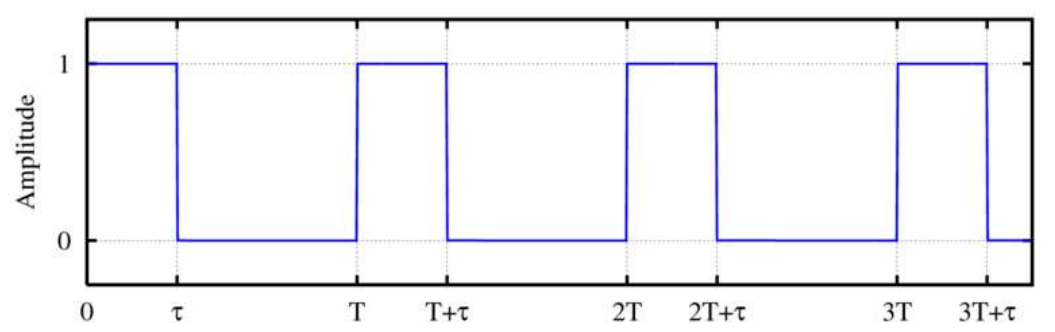
\includegraphics[width=1\columnwidth]{images/rect.png}
    \caption{A periodic rectangular waveform with frequency $1/T$ and a duty cycle of $\tau/T \cross 100\%$}
    \label{rect}
\end{figure}

\subsubsection{With duty cycle more than 50\%}
An astable
multivibrator can be designed as shown in the circuit diagram (with typical component
values) using IC 555, for a duty cycle of more than 50\%. The corresponding voltage
across the capacitor and voltage at output is also shown. The astable function is achieved
by charging/discharging a capacitor through resistors connected, respectively, either to
$V_{CC}$ or GND. Switching between the charging and discharging modes is handled by
resistor divider $R_1-R_3$, two Comparators, and an RS Flip-Flop in IC 555. The upper or
lower comparator simply generates a positive pulse if $V_{CC}$ goes above 2/3 $V_{CC}$ or below
1/3 $V_{CC}$. And these positive pulses either \verb|SET| or \verb|RESET| the Q output.

\begin{figure}[H]
    \centering
    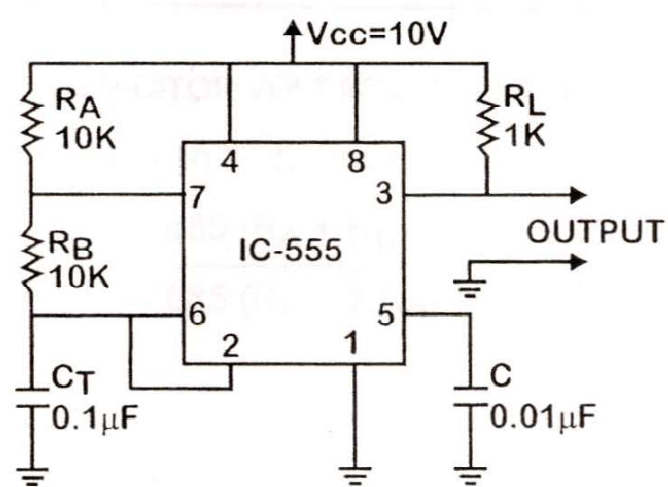
\includegraphics[width=0.7\columnwidth]{images/ast.png}
    \caption{Circuit diagram of an astable multivibrator with duty cycle more than 50\%}
    \label{ast}
\end{figure}

\noindent The time for charging C from $1/3$ to $2/3$ $V_{CC}$ (ON) 
\begin{align*}
    = 0.693\,(R_A+R_B)\,C
\end{align*}

The time for discharging C from $2/3$ to $1/3$ $V_{CC}$ (OFF)
\begin{align*}
    = 0.693\,R_B\,C
\end{align*}    
The total oscillation period,

\begin{align}
    T_\text{osc} &= 0.693\,(R_A+2R_B)\,C \nonumber\\
    \implies f_\text{osc} &= \frac{1.44}{(R_A+2R_B)C}\\
    \text{and, Duty Cycle} &= \frac{R_A+R_B}{R_A+2R_B}
\end{align}

\begin{figure}[H]
    \centering
    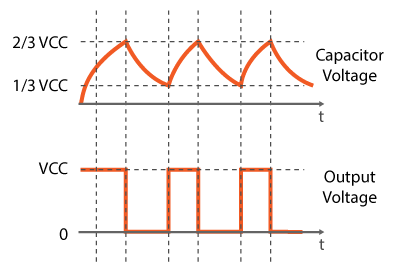
\includegraphics[width=0.90\columnwidth]{images/ast2.png}
    \caption{The voltage across the capacitor compared with the output voltage across time (for an arbitrary duty cycle)}
    \label{ast2}
\end{figure}

\subsubsection{With duty cycle less than 50\%}
Here a diode $D_1$ is connected between the discharge and threshold terminals (as also
across RB). Thus the capacitor now charges only through $R_A$ (since $R_B$ is shorted by diode
conduction during charging) and discharges through $R_B$. Another optional diode $D_2$ is
also connected in series with $R_B$ in reverse direction for better shorting of $R_B$. Therefore,
the frequency of oscillation and duty cycle are

\begin{align}
    f_\text{osc} &= \frac{1.44}{(R_A+R_B)C}\\
    \text{Duty Cycle} &= \frac{R_A}{R_A+2R_B}
\end{align}

\begin{figure}[H]
    \centering
    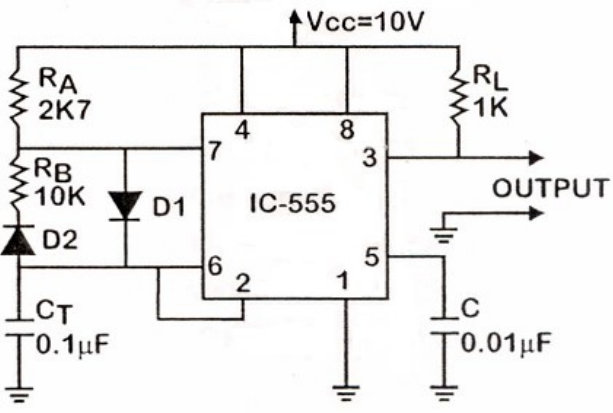
\includegraphics[width=0.7\columnwidth]{images/ast3.png}
    \caption{Circuit diagram of an astable multivibrator with duty cycle less than 50\%}
    \label{ast3}
\end{figure}

\subsubsection{With duty cycle variable from 0 to 100\%}
Here a potentiometer, $R_X$, is
used so that $R_A = R_1+R_2$, $R_B = R_X-R_2+R_3$. A diode is now connected across a variable $R_B$.
Thus a variable duty cycle is achieved. Therefore, the frequency of oscillation and duty
cycle can be derived as follows.
\begin{align}
    f_\text{osc} &= \frac{1.44}{(R_1+R_X+R_3)C}\\
    \text{Min. Duty Cycle} &= \frac{R_1}{R_1+R_X+R_3}\\
    \text{Max. Duty Cycle} &= \frac{R_1+R_X}{R_1+R_X+R_3}
\end{align}

\begin{figure}[H]
    \centering
    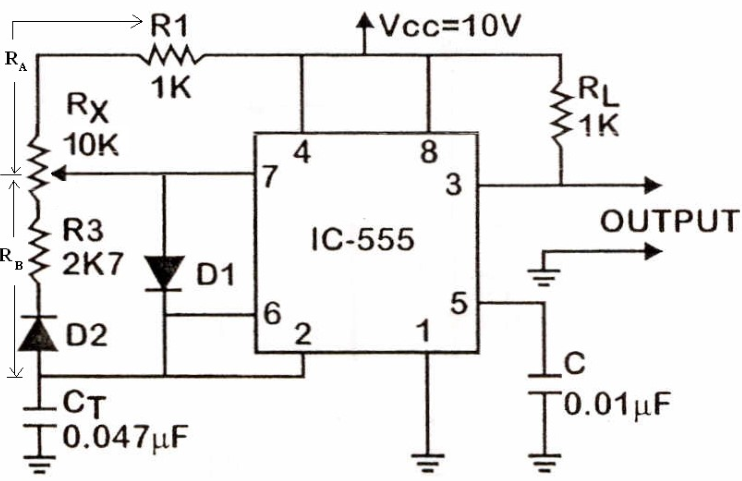
\includegraphics[width=0.7\columnwidth]{images/ast4.png}
    \caption{Circuit diagram of an astable multivibrator with variable duty cycle from 0 to 100\%}
    \label{ast4}
\end{figure}

\subsection{Monostable Multivibrator}

Monostable multivibrator or a one shot multivibrator is a pulse generating
circuit where the duration of this pulse is determined by the RC network connected
externally. When a negative pulse is applied to the trigger input (pin 2) of the Monostable oscillator, the internal comparator, detects this input and “sets” the state of the flip-flop, changing the output from a \verb|LOW| state to a \verb|HIGH| state. This action turns “OFF” the discharge transistor connected to pin 7, removing the short circuit across the external timing capacitor, C.

This allows the timing capacitor to start to charge up through resistor, R until the voltage across the capacitor reaches the threshold (pin 6) voltage of $2/3$ $V_{CC}$ set up by the internal voltage divider network. At this point the comparator's output goes \verb|HIGH| and “resets” the flip-flop back to its original state which in turn turns “ON” the transistor and discharges the capacitor to ground through pin 7. This causes the output to change its state back to the original stable \verb|LOW| value awaiting another trigger pulse to start the timing process over again. Then as before, the Monostable Multivibrator has only 1 stable state.

\begin{figure}[H]
    \centering
    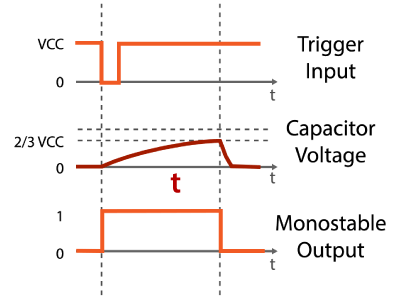
\includegraphics[width=0.6\columnwidth]{images/mono1.png}
    \caption{The voltage across the capacitor compared with the output voltage and the input trigger across time}
    \label{mono1}
\end{figure}

The Monostable 555 Timer circuit triggers on a negative-going pulse applied to pin 2 and this trigger pulse must be much shorter than the output pulse width allowing time for the timing capacitor to charge and then discharge fully. Once triggered, the 555 Monostable will remain in this \verb|HIGH| unstable output state until the time period set up by the $R C$ network has elapsed. The amount of time that the output voltage remains \verb|HIGH| or at a logic 1 level, is given by the following time constant equation,

\begin{align}
    T=1.1\,RC
\end{align}

\begin{figure}[H]
    \centering
    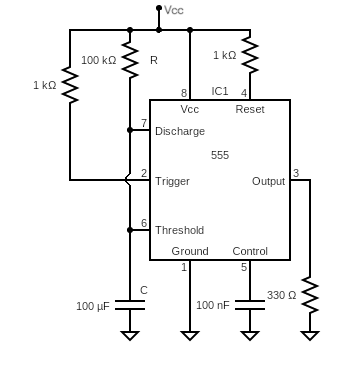
\includegraphics[width=0.65\columnwidth]{images/mono2.png}
    \caption{Circuit diagram of a monostable multivibrator}
    \label{mono2}
\end{figure}

\subsection{Bistable Multivibrator}
In these circuits, the output is stable in both states. The states are switched using an
external trigger but unlike the monostable multivibrator, it does not return back to its
original state. Another trigger is needed for this to happen. This operation is similar to a
flip-flop. There are no RC timing networks and hence no design parameters. The
following circuit can be used to design a bistable multivibrator. The trigger and reset
inputs (pins 2 and 4 respectively on a 555) are held high via pull-up resistors while the
threshold input (pin 6) is simply grounded. Thus configured, pulling the trigger
momentarily to ground acts as a \verb|SET| and transitions the output pin (pin 3) to $V_{CC}$ (high
state). Pulling the threshold input to supply acts as a \verb|RESET| and transitions the output pin
to ground (low state). 

\begin{figure}[H]
    \centering
    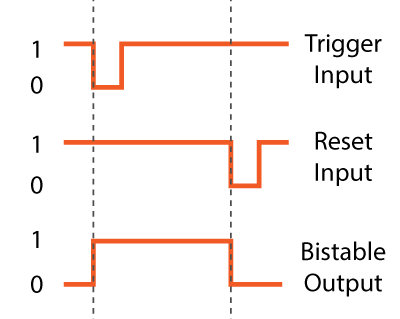
\includegraphics[width=0.5\columnwidth]{images/bis1.png}
    \caption{The input and reset triggers along with the multivibrator output voltage waveforms}
    \label{bis1}
\end{figure}

\begin{figure}[H]
    \centering
    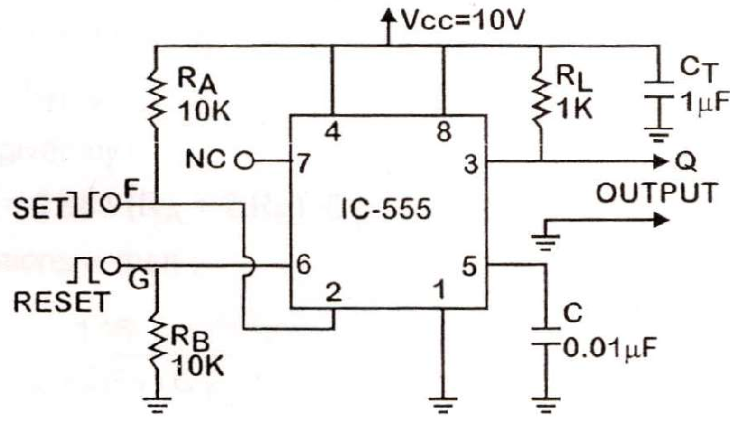
\includegraphics[width=0.8\columnwidth]{images/bis2.png}
    \caption{Circuit diagram of a bistable multivibrator}
    \label{bis2}
\end{figure}

% ======================================================================================
\section{Apparatus}

\begin{enumerate}
    \item IC 555
    \item Resistors
    \item Potentiometer
    \item Capacitors
    \item Diodes
    \item Multimeters
    \item Oscilloscope
    \item D.C. Power Supply (10V)
    \item Connecting Wires
    \item Breadboard
\end{enumerate}